% ROZDZIAŁ 10 — do włączenia w main.tex
\chapter[Regularność funkcji mierzalnych]{Regularność funkcji mierzalnych i aproksymacja funkcjami ciągłymi}
\label{ch:regularnosc-funkcji}

\section{Co oznacza regularność funkcji mierzalnej?}

Funkcja mierzalna może być nieciągła we wszystkich punktach,
jak funkcja Dirichleta. Mimo to mierzalność jest blisko
związana z ciągłością \emph{w sensie miary}: na zbiorze o
skończonej mierze można usunąć zbiór o dowolnie małej mierze
i otrzymać ciągłość na pozostałym odpowiednio dobranym
zbiorze zwartym. Taką treść ma twierdzenie Łuzina.

W odróżnieniu od twierdzenia Jegorowa, które dotyczy
zbieżności \emph{ciągu} funkcji, twierdzenie Łuzina
przybliża pojedynczą funkcję mierzalną przez funkcje
ciągłe. Oba twierdzenia współpracują: najpierw
aproksymujemy funkcję mierzalną funkcjami prostymi,
a następnie wymuszamy jednostajność zbieżności
poza niewielkim zbiorem wyjątkowym.

W całym rozdziale $d\ge1$ i $\lambda_d$ oznacza miarę
Lebesgue'a na $\mathbb R^d$. Przez $\mathcal L_d$
oznaczamy jej $\sigma$-algebrę zbiorów mierzalnych.
Topologię na podzbiorach $\mathbb R^d$ rozumiemy jako
topologię podprzestrzeni. W szczególności sformułowanie
``$f|_K$ jest ciągła'' \emph{nie} oznacza,
że $f$ jest ciągła w punktach $K$ jako funkcja na
całej dziedzinie.

\begin{uwaga}[Dwa różne symbole]
Funkcję charakterystyczną zbioru $A$ oznaczamy
wyłącznie przez $\chi_A$. Gładkie funkcje odcinające
oznaczamy literą $\vartheta$ lub $\psi$; nie są one
funkcjami charakterystycznymi i przyjmują na ogół
również wartości pośrednie między zerem a jedynką.
\end{uwaga}

\section{Dwa narzędzia: regularność miary i funkcje odcinające}

\begin{lemat}[Przybliżenie mierzalnego zbioru przez zbiór zwarty]
\label{lem:compact-inside-10}
Niech $A\in\mathcal L_d$ oraz $\lambda_d(A)<\infty$.
Dla każdego $\varepsilon>0$ istnieją zbiór
zwarty $K$ i zbiór otwarty $O$ w $\mathbb R^d$ takie,
że $K\subseteq A\subseteq O$ i
\begin{equation}\label{eq:compact-open-10}
\lambda_d(O\setminus K)<\varepsilon.
\end{equation}
\end{lemat}
\begin{proof}
Regularność wewnętrzna miary Lebesgue'a daje
zwarty $K\subseteq A$ z
$\lambda_d(A\setminus K)<\varepsilon/2$.
Regularność zewnętrzna daje otwarty $O\supseteq A$
z $\lambda_d(O\setminus A)<\varepsilon/2$.
Ponieważ $O\setminus K$ jest rozłączną sumą
$(O\setminus A)\cup(A\setminus K)$,
addytywność miary daje \eqref{eq:compact-open-10}.
Jeśli chcemy jedynie otrzymać otwarte otoczenie
zbioru zwartego $K$ o małej różnicy miar,
możemy je dodatkowo wybrać ograniczone:
wystarczy przeciąć $O$ z kulą zawierającą $K$.
\end{proof}

\begin{uwaga}[Niedopuszczalna zamiana kwantyfikatorów]
Zbiór zwarty $K$ zależy od $\varepsilon$.
Na ogół nie istnieje jeden zbiór zwarty zawierający
wszystkie poza mierzalnym zbiorem zerowym punkty
$A$ (w szczególności gdy $A$ nie jest ograniczony).
Nie wolno również zastępować założenia
$\lambda_d(A)<\infty$ samym założeniem
$A\in\mathcal L_d$ w żądaniu
$\lambda_d(A\setminus K)<\varepsilon$.
\end{uwaga}

\begin{lemat}[Gładka funkcja odcinająca]
\label{lem:smooth-cutoff-10}
Niech $K\subseteq\mathbb R^d$ będzie zwarty,
a $O\subseteq\mathbb R^d$ otwarty i zawierający $K$.
Istnieje funkcja $\vartheta\in C_c^\infty(\mathbb R^d)$
taka, że $0\le\vartheta\le1$, $\vartheta=1$ na $K$
oraz $\operatorname{supp}\vartheta\subseteq O$.
Przez $\operatorname{supp}\vartheta$ rozumiemy domknięcie
zbioru $\{\vartheta\ne0\}$, a $C_c^\infty$ oznacza
funkcje gładkie o zwartym nośniku.
\end{lemat}
\begin{proof}
Jeśli $K=\varnothing$, bierzemy $\vartheta=0$.
W przeciwnym razie dla każdego $a\in K$ wybieramy
$r_a>0$ tak, żeby $\overline{B(a,r_a)}\subseteq O$.
Zwartość $K$ pozwala wybrać skończenie wiele
kul $B(a_j,r_j/2)$ pokrywających $K$.

Niech $\eta:\mathbb R\to[0,\infty)$ będzie określona
wzorem $\eta(t)=e^{-1/t}$ dla $t>0$ i $\eta(t)=0$
dla $t\le0$. Wzór ten określa funkcję klasy
$C^\infty$; każda jej pochodna dla $t>0$ jest
sumą wyrazów $P(1/t)e^{-1/t}$ i ma granicę zero
przy $t\downarrow0$, co dowodzi gładkości także
w zerze. Zdefiniujmy
\[
\psi_j(x)=
\frac{\eta(r_j^2-|x-a_j|^2)}
{\eta(r_j^2-|x-a_j|^2)+
 \eta(|x-a_j|^2-r_j^2/4)}.
\]
Mianownik jest dodatni dla każdego $x$:
dla $|x-a_j|<r_j$ dodatni jest pierwszy składnik,
a dla $|x-a_j|\ge r_j$ drugi. Widzimy, że
$\psi_j=1$ na $\overline{B(a_j,r_j/2)}$,
$\psi_j=0$ poza $B(a_j,r_j)$ i
$0\le\psi_j\le1$.
Kładziemy $\vartheta=1-\prod_j(1-\psi_j)$.
Jest gładka, równa $1$ na $K$ i ma nośnik zawarty
w skończonej sumie zwartych kul
$\overline{B(a_j,r_j)}\subseteq O$.
\end{proof}

\begin{wniosek}[Przybliżanie funkcji charakterystycznej]
\label{cor:indicator-smooth-10}
Niech $A\in\mathcal L_d$ i $\lambda_d(A)<\infty$.
Dla każdego $1\le p<\infty$ i $\varepsilon>0$
istnieje $\vartheta\in C_c^\infty(\mathbb R^d)$ taka,
że $0\le\vartheta\le1$ oraz
\begin{equation}\label{eq:indicator-smooth-10}
\int_{\mathbb R^d}|\chi_A(x)-\vartheta(x)|^p
\,\mathrm d\lambda_d(x)<\varepsilon.
\end{equation}
\end{wniosek}
\begin{proof}
Z lematu \ref{lem:compact-inside-10} wybieramy
$K\subseteq A\subseteq O$ z
$\lambda_d(O\setminus K)<\varepsilon$.
Stosujemy lemat \ref{lem:smooth-cutoff-10}.
Na $K$ funkcje $\chi_A$ i $\vartheta$ są równe $1$,
a poza $O$ są równe $0$. Na pozostałym zbiorze
$O\setminus K$ ich różnica ma moduł co najwyżej $1$.
Stąd całka po $\mathbb R^d$ jest ograniczona przez
$\lambda_d(O\setminus K)<\varepsilon$.
\end{proof}

\begin{center}
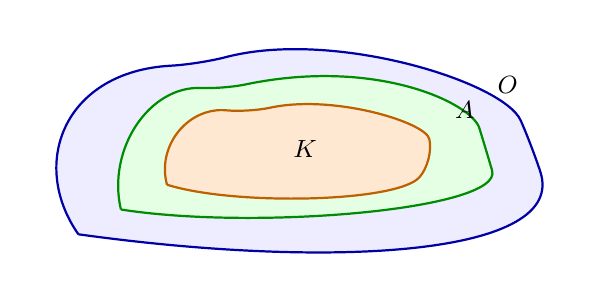
\begin{tikzpicture}[scale=.9,every node/.style={font=\small}]
\draw[rounded corners=10pt,thick,fill=blue!7,draw=blue!65!black]
(0,0) .. controls (-.7,1) and (-.2,2.3) .. (1.7,2.4)
.. controls (3.6,2.9) and (6,2.15) .. (6.4,1.25)
.. controls (6.9,-.3) and (3.6,-.5) .. (0,0);
\draw[rounded corners=8pt,thick,fill=green!10,draw=green!55!black]
(.6,.35) .. controls (.4,1.2) and (1,2.1) .. (2.05,2.05)
.. controls (4.2,2.5) and (5.55,1.85) .. (5.75,1.2)
.. controls (6,.35) and (2.5,.05) .. (.6,.35);
\draw[rounded corners=8pt,thick,fill=orange!18,draw=orange!75!black]
(1.25,.7) .. controls (1.1,1.25) and (1.55,1.8) .. (2.4,1.72)
.. controls (3.6,1.98) and (4.9,1.58) .. (5.02,1.04)
.. controls (4.5,.45) and (2.2,.4) .. (1.25,.7);
\node at (3.2,1.2) {$K$};
\node at (5.45,1.75) {$A$};
\node at (6.06,2.10) {$O$};
\end{tikzpicture}
\par\smallskip
\textit{Schemat regularności miary: $K\subseteq A\subseteq O$,
przy czym $\lambda_d(O\setminus K)$ jest dowolnie mała.
Rysunek ma charakter poglądowy.}
\end{center}

\section{Funkcje proste ciągłe na dużym zbiorze zwartym}

\begin{lemat}[Łuzin dla funkcji prostych]
\label{lem:lusin-simple-10}
Niech $E\in\mathcal L_d$, $\lambda_d(E)<\infty$,
a $s:E\to\mathbb R$ będzie mierzalną funkcją prostą.
Dla każdego $\varepsilon>0$ istnieje zwarty
$K\subseteq E$ taki, że
$\lambda_d(E\setminus K)<\varepsilon$ oraz
$s|_K$ jest ciągła.
\end{lemat}
\begin{proof}
Jeżeli $E=\varnothing$, bierzemy $K=\varnothing$;
ograniczenie $s|_K$ jest ciągłe, a
$\lambda_d(E\setminus K)=0<\varepsilon$.
Dalej zakładamy $E\ne\varnothing$, zatem liczba
różnych wartości $m$ jest dodatnia.
Niech $a_1,\dots,a_m$ będą różnymi wartościami $s$
i $A_j=\{x\in E:s(x)=a_j\}$.
Są to parami rozłączne zbiory mierzalne, których
suma jest równa $E$. Wszystkie mają skończoną miarę.
Dla każdego $j$ regularność wewnętrzna daje
zwarty $K_j\subseteq A_j$ taki, że
$\lambda_d(A_j\setminus K_j)<\varepsilon/m$.
Zbiór $K=\bigcup_{j=1}^mK_j$ jest zwarty,
$K\subseteq E$ i
$\lambda_d(E\setminus K)<\varepsilon$.

Ponieważ zbiory $K_j$ są parami rozłączne i zwarte,
każdy z nich jest otwarty i domknięty w podprzestrzeni
$K$: jego dopełnienie w $K$ jest skończoną sumą
zbiorów zwartych, a więc domkniętych.
Funkcja $s|_K$, stała na każdym z tych zbiorów,
jest zatem ciągła. Nie wyciągamy błędnego wniosku,
że $s$ jest ciągła na całym $E$.
\end{proof}

\section{Twierdzenie Łuzina}

\begin{twierdzenie}[Łuzin]
\label{thm:lusin-10}
Niech $E\in\mathcal L_d$ będzie zbiorem o
$\lambda_d(E)<\infty$, a $f:E\to\mathbb R$
funkcją mierzalną względem śladu
$\mathcal L_d|_E$. Wtedy dla każdego
$\varepsilon>0$ istnieje zwarty zbiór
$K\subseteq E$ taki, że
\begin{equation}\label{eq:lusin-measure-10}
\lambda_d(E\setminus K)<\varepsilon
\end{equation}
oraz $f|_K:K\to\mathbb R$ jest ciągła.
\end{twierdzenie}
\begin{proof}
\textit{Krok 1: aproksymacja funkcją prostą.}
Na mocy twierdzenia o aproksymacji funkcji
mierzalnych z rozdziału 6 istnieją mierzalne
funkcje proste $s_n:E\to\mathbb R$ takie, że
$s_n(x)\to f(x)$ dla każdego $x\in E$.
Możemy na przykład stosować obcięcia wartości
$f$ i ich kwantyzację na przedziałach długości
$2^{-n}$, najpierw do części dodatniej i ujemnej.
Nie korzystamy w tym kroku z twierdzenia Łuzina.

\textit{Krok 2: prawie jednostajność.}
Ponieważ $\lambda_d(E)<\infty$, twierdzenie
Jegorowa \ref{thm:egorov-9}, zastosowane do
przestrzeni z miarą $E$, daje mierzalny zbiór
$Z\subseteq E$ taki, że
$\lambda_d(Z)<\varepsilon/4$ i $s_n\to f$
jednostajnie na $E\setminus Z$.
Z regularności wewnętrznej wybieramy zwarty
$K_0\subseteq E\setminus Z$, dla którego
$\lambda_d((E\setminus Z)\setminus K_0)<\varepsilon/4$.
Na $K_0$ zbieżność jest jednostajna.

\textit{Krok 3: ciągłość wszystkich przybliżeń.}
Dla każdego $n\ge1$ stosujemy lemat
\ref{lem:lusin-simple-10} do $s_n$ na $E$
z tolerancją $\varepsilon 2^{-(n+2)}$.
Otrzymujemy zwarty $K_n\subseteq E$ taki, że
$\lambda_d(E\setminus K_n)<
\varepsilon2^{-(n+2)}$ i $s_n|_{K_n}$ jest ciągła.
Kładziemy
$K=K_0\cap\bigcap_{n\ge1}K_n$.
Jest to zbiór zwarty jako domknięty podzbiór
zbioru zwartego $K_0$. Ponadto
\[
\lambda_d(E\setminus K)
\le\lambda_d(Z)+
\lambda_d((E\setminus Z)\setminus K_0)+
\sum_{n\ge1}\lambda_d(E\setminus K_n)
<\frac\varepsilon4+\frac\varepsilon4+
\frac\varepsilon4<\varepsilon.
\]
Dla każdego $n$ funkcja $s_n|_K$ jest ciągła,
a ciąg $(s_n|_K)$ zbiega jednostajnie do $f|_K$.
Jednostajna granica funkcji ciągłych na przestrzeni
metrycznej jest ciągła; stąd $f|_K$ jest ciągła.
\end{proof}

\begin{wniosek}[Funkcje skończone prawie wszędzie]
\label{cor:lusin-finite-ae-10}
Niech $E\in\mathcal L_d$ ma skończoną miarę,
a $f:E\to\overline{\mathbb R}$ jest mierzalna względem
śladu $\mathcal L_d|_E$ i skończona $\lambda_d$-prawie
wszędzie. Dla każdego $\varepsilon>0$ istnieje
zwarty $K\subseteq E$ taki, że
$\lambda_d(E\setminus K)<\varepsilon$ oraz
$f|_K:K\to\mathbb R$ jest ciągła.
\end{wniosek}
\begin{proof}
Zbiór $N=\{x\in E:|f(x)|=\infty\}$ jest
mierzalny i zerowy. Na $E\setminus N$ funkcja
jest rzeczywista i mierzalna. Stosujemy twierdzenie
Łuzina do $E\setminus N$, którego miara jest
równa $\lambda_d(E)$. Otrzymany zwarty
$K\subseteq E\setminus N$ ma żądane własności.
\end{proof}

\begin{wniosek}[Jednoczesne twierdzenie Łuzina dla przeliczalnej rodziny]
\label{cor:countable-lusin-10}
Niech $E\in\mathcal L_d$ ma skończoną miarę,
a $f_j:E\to\mathbb R$, $j\ge1$, będą
funkcjami mierzalnymi. Dla każdego $\varepsilon>0$
istnieje zwarty $K\subseteq E$ taki, że
$\lambda_d(E\setminus K)<\varepsilon$ i
\emph{wszystkie} ograniczenia $f_j|_K$ są ciągłe.
\end{wniosek}
\begin{proof}
Dla każdego $j$ stosujemy twierdzenie Łuzina
z tolerancją $\varepsilon2^{-(j+1)}$.
Otrzymujemy zwarte $K_j\subseteq E$ takie,
że $\lambda_d(E\setminus K_j)<\varepsilon2^{-(j+1)}$
i $f_j|_{K_j}$ jest ciągła.
Zbiór $K=\bigcap_{j\ge1}K_j$ jest zwarty
(jako domknięty podzbiór $K_1$), a
\[
\lambda_d(E\setminus K)
\le\sum_{j\ge1}\lambda_d(E\setminus K_j)
<\varepsilon.
\]
Każda $f_j|_K$ jest ciągła jako ograniczenie
funkcji ciągłej na $K_j$.
\end{proof}

\begin{uwaga}[Granice twierdzenia]
\label{rem:lusin-limitations-10}
Twierdzenie Łuzina nie orzeka, że $f$ jest
ciągła \emph{w punktach} $K$ względem całej
dziedziny $E$. Na przykład $f=\chi_{\mathbb Q}$
na $[0,1]$ jest nieciągła w każdym punkcie, ale
jej ograniczenie do dowolnego zbioru zwartego
niezawierającego liczb wymiernych jest funkcją
stałą, a więc ciągłą. Możemy znaleźć takie
zbiory zwarte o mierze dowolnie bliskiej $1$.

Skończoność miary $E$ jest istotna w podanej formie.
Dla $E=\mathbb R^d$ żaden zwarty podzbiór $K$
nie spełnia $\lambda_d(E\setminus K)<1$,
niezależnie od wyboru funkcji $f$.
\end{uwaga}

\section{Przedłużanie funkcji ciągłej ze zbioru zwartego}

\begin{lemat}[Lipschitzowska aproksymacja na zbiorze zwartym]
\label{lem:lipschitz-approx-compact-10}
Niech $K\subseteq\mathbb R^d$ będzie niepustym
zbiorem zwartym, a $h:K\to\mathbb R$ funkcją ciągłą.
Dla każdego $\varepsilon>0$ istnieje ograniczona
funkcja Lipschitzowska $H:\mathbb R^d\to\mathbb R$
taka, że
$\sup_{x\in K}|H(x)-h(x)|<\varepsilon$
i $\sup_{\mathbb R^d}|H|\le\sup_K|h|$.
\end{lemat}
\begin{proof}
Niech $M=\sup_K|h|<\infty$. Jeśli $M=0$,
wystarczy $H=0$. W przeciwnym razie z jednostajnej
ciągłości $h$ na $K$ wybieramy $\delta>0$ takie, że
$|h(x)-h(y)|<\varepsilon/2$ przy
$x,y\in K$, $|x-y|<\delta$.
Wybieramy $L>2M/\delta$ i definiujemy na
całym $\mathbb R^d$
\[
U_L(x)=\inf_{y\in K}\bigl(h(y)+L|x-y|\bigr).
\]
Dla dowolnych $x,z\in\mathbb R^d$ z nierówności
$|x-y|\le|x-z|+|z-y|$ wynika
$U_L(x)\le U_L(z)+L|x-z|$. Zamieniając $x,z$,
dostajemy $|U_L(x)-U_L(z)|\le L|x-z|$.

Dla $x\in K$ mamy $U_L(x)\le h(x)$ (wybierając
$y=x$). Jeśli $|y-x|<\delta$, to
$h(y)+L|x-y|>h(x)-\varepsilon/2$.
Jeżeli $|y-x|\ge\delta$, to
$h(y)+L|x-y|\ge-M+L\delta>M\ge h(x)$.
Wynika $h(x)-\varepsilon/2\le U_L(x)\le h(x)$.
Funkcja
$H(x)=\max(-M,\min(M,U_L(x)))$
jest ograniczona i Lipschitzowska, a obcięcie do
$[-M,M]$ nie zwiększa błędu na $K$.
\end{proof}

\begin{twierdzenie}[Przedłużenie z kompaktu w $\mathbb R^d$]
\label{thm:compact-extension-10}
Jeśli $K\subseteq\mathbb R^d$ jest zwarty,
a $h:K\to\mathbb R$ ciągła, to istnieje
$H\in C(\mathbb R^d)$ taka, że $H|_K=h$.
Można dodatkowo wymagać
$\sup_{\mathbb R^d}|H|\le\sup_K|h|$
dla $K\ne\varnothing$. Jeśli $K=\varnothing$,
wybieramy $H=0$; nie używamy wtedy supremum
rzeczywistych wartości funkcji na zbiorze pustym.
\end{twierdzenie}
\begin{proof}
Przy $K=\varnothing$ bierzemy $H=0$.
Niech $K\ne\varnothing$ i $M_0=\sup_K|h|$.
Konstruujemy funkcje Lipschitzowskie $u_n$ i
reszty $r_n:K\to\mathbb R$ rekurencyjnie.
Kładziemy $r_0=h$. Jeśli
$M_n=\sup_K|r_n|>0$, stosujemy lemat
\ref{lem:lipschitz-approx-compact-10} z błędem
$M_n/2$, uzyskując $u_n$ o
$\sup_{\mathbb R^d}|u_n|\le M_n$ i
$\sup_K|u_n-r_n|<M_n/2$.
Definiujemy $r_{n+1}=r_n-u_n|_K$.
Wtedy $M_{n+1}\le M_n/2$. Jeśli $M_n=0$,
bierzemy $u_n=0$ i wszystkie dalsze reszty
równe zero.

Z oszacowania
$\sup_{\mathbb R^d}|u_n|\le M_0 2^{-n}$
wynika jednostajna zbieżność szeregu
$G=\sum_{n\ge0}u_n$ na całym $\mathbb R^d$.
Jest to funkcja ciągła. Na $K$ mamy dla każdego
$N$ tożsamość
$h=\sum_{n=0}^Nu_n|_K+r_{N+1}$;
po przejściu do granicy otrzymujemy $G|_K=h$.
Na koniec funkcja $H=\max(-M_0,\min(M_0,G))$
pozostaje ciągła, zgadza się z $h$ na $K$
i ma żądane ograniczenie.
\end{proof}

\begin{wniosek}[Wersja Łuzina przez funkcję ciągłą na całej przestrzeni]
\label{cor:lusin-extension-10}
Niech $E\in\mathcal L_d$, $\lambda_d(E)<\infty$,
i $f:E\to\mathbb R$ będzie mierzalna. Dla każdego
$\varepsilon>0$ istnieją $K\subseteq E$ zwarty
i $H\in C(\mathbb R^d)$ takie, że
$\lambda_d(E\setminus K)<\varepsilon$ oraz
$H(x)=f(x)$ dla wszystkich $x\in K$.
\end{wniosek}
\begin{proof}
Stosujemy twierdzenie \ref{thm:lusin-10},
a następnie twierdzenie \ref{thm:compact-extension-10}
do funkcji ciągłej $f|_K$.
\end{proof}

\section{Aproksymacja w mierze przez funkcje ciągłe i gładkie}

\begin{twierdzenie}[Aproksymacja funkcji o nośniku mierzalnym skończonej miary]
\label{thm:cc-approx-in-measure-10}
Niech $E\in\mathcal L_d$, $\lambda_d(E)<\infty$,
i niech $f:E\to\mathbb R$ będzie mierzalna.
Przedłużmy $f$ zerem poza $E$, otrzymując
$\widetilde f:\mathbb R^d\to\mathbb R$.
Dla każdych $\varepsilon,\delta>0$ istnieje
$\varphi\in C_c(\mathbb R^d)$ takie, że
\begin{equation}\label{eq:cc-approx-measure-10}
\lambda_d\bigl(\{x\in\mathbb R^d:
|\widetilde f(x)-\varphi(x)|>\delta\}\bigr)
<\varepsilon.
\end{equation}
Można dodatkowo wybrać $\varphi$ tak, aby
$\varphi=\widetilde f$ \emph{dokładnie} na pewnym
zbiorze zwartym $K\subseteq E$ z
$\lambda_d(E\setminus K)<\varepsilon/2$.
\end{twierdzenie}
\begin{proof}
Z twierdzenia Łuzina wybieramy zwarty
$K\subseteq E$ taki, że
$\lambda_d(E\setminus K)<\varepsilon/2$
oraz $f|_K$ jest ciągła.
Z regularności zewnętrznej \emph{zbioru zwartego}
$K$ wybieramy otwarty $O$ zawierający $K$ tak,
że $\lambda_d(O\setminus K)<\varepsilon/2$.
Nie musimy wymagać, aby $O$ zawierał całe $E$.

Przedłużamy $f|_K$ do funkcji ciągłej
$H:\mathbb R^d\to\mathbb R$ na mocy
\ref{thm:compact-extension-10}. Na mocy lematu
\ref{lem:smooth-cutoff-10} istnieje
$\vartheta\in C_c^\infty(\mathbb R^d)$, $\vartheta=1$ na $K$,
z $\operatorname{supp}\vartheta\subseteq O$.
Kładziemy $\varphi=\vartheta H$. Wtedy
$\varphi\in C_c(\mathbb R^d)$ i na $K$ zachodzi
$\varphi=f$. Poza $E\cup O$ obie funkcje
$\varphi$ i $\widetilde f$ są zerowe. Stąd
zbiór, na którym funkcje mogą się różnić,
jest zawarty w $(E\setminus K)\cup(O\setminus K)$,
a jego miara jest mniejsza niż $\varepsilon$.
Implikuje to \eqref{eq:cc-approx-measure-10}
dla każdego $\delta>0$.
\end{proof}

\begin{uwaga}[Dlaczego nie istnieje takie twierdzenie dla dowolnego $f$ na $\mathbb R^d$?]
Dla funkcji $f\equiv1$ na $\mathbb R^d$ i dowolnej
$\varphi\in C_c(\mathbb R^d)$ zbiór
$\{|f-\varphi|>1/2\}$ zawiera dopełnienie
zwartego nośnika $\varphi$, a więc ma nieskończoną
miarę Lebesgue'a. Założenie o skończonej mierze
zbioru podtrzymującego funkcję nie jest czysto
technicznym dodatkiem.
\end{uwaga}

\begin{lemat}[Wygładzanie funkcji ciągłej o zwartym nośniku]
\label{lem:mollify-cc-10}
Niech $h\in C_c(\mathbb R^d)$. Istnieje ciąg
$h_n\in C_c^\infty(\mathbb R^d)$ taki, że
$\sup_{x\in\mathbb R^d}|h_n(x)-h(x)|\to0$.
\end{lemat}
\begin{proof}
Z lematu \ref{lem:smooth-cutoff-10} otrzymujemy
nieujemną, niezerową funkcję
$\rho\in C_c^\infty(\mathbb R^d)$ o nośniku
zawartym w kuli $B(0,1)$. Po podzieleniu przez
$\int_{\mathbb R^d}\rho(x)\,\mathrm d\lambda_d(x)>0$
możemy przyjąć, że ta całka jest równa $1$.
Dla $t>0$ określamy
$\rho_t(x)=t^{-d}\rho(x/t)$ oraz
\[
h_t(x)=\int_{\mathbb R^d}
 h(y)\rho_t(x-y)\,\mathrm d\lambda_d(y).
\]
Z niezmienniczości i skalowania miary Lebesgue'a
(rozdział 4) wynika
$\int_{\mathbb R^d}\rho_t(x-y)\,\mathrm d\lambda_d(y)=1$.

Funkcja $h_t$ ma nośnik zawarty w
$\operatorname{supp}h+\overline{B(0,t)}$,
który jest zwarty. Jest gładka: pochodne względem
$x$ dowolnego rzędu można przenosić pod znak
całki dzięki ograniczoności pochodnych $\rho_t$
i temu, że integrujemy po ustalonym zwartym
nośniku $h$. Formalnie stosujemy iteracyjnie
twierdzenie o różniczkowaniu pod znakiem całki
z rozdziału 8, osobno do każdej współrzędnej.

Ponadto dla każdego $x$ mamy
\[
|h_t(x)-h(x)|
\le\int_{\mathbb R^d}|h(y)-h(x)|\rho_t(x-y)
\,\mathrm d\lambda_d(y)
\le\sup_{|x-y|\le t}|h(y)-h(x)|.
\]
Funkcja $h$ jest jednostajnie ciągła na
$\mathbb R^d$, bo jest ciągła i ma zwarty nośnik.
Ostatnie supremum dąży jednostajnie do zera dla
$t\downarrow0$. Wybieramy $h_n=h_{1/n}$.
\end{proof}

\begin{wniosek}[Aproksymacja w mierze funkcjami gładkimi]
\label{cor:smooth-approx-in-measure-10}
Niech $E\in\mathcal L_d$ ma skończoną miarę
i niech $f:E\to\mathbb R$ będzie mierzalna
względem śladu. Oznaczmy przez
$\widetilde f:\mathbb R^d\to\mathbb R$
przedłużenie funkcji $f$ zerem poza $E$.
Dla dowolnych $\varepsilon,\delta>0$ istnieje
$\psi\in C_c^\infty(\mathbb R^d)$ taka, że
\[
\lambda_d\bigl(\{|\widetilde f-\psi|>\delta\}\bigr)
<\varepsilon.
\]
\end{wniosek}
\begin{proof}
Z twierdzenia \ref{thm:cc-approx-in-measure-10}
wybieramy $\varphi\in C_c(\mathbb R^d)$ taką,
że $\lambda_d(\{|\widetilde f-\varphi|>
\delta/2\})<\varepsilon$.
Z lematu \ref{lem:mollify-cc-10} wybieramy
$\psi\in C_c^\infty$ taką, że
$\sup|\psi-\varphi|<\delta/2$.
Wtedy
$\{|\widetilde f-\psi|>\delta\}\subseteq
\{|\widetilde f-\varphi|>\delta/2\}$.
\end{proof}

\section{Gęstość $C_c^\infty$ w przestrzeniach $L^p$}

\begin{twierdzenie}[Gęstość funkcji gładkich]
\label{thm:cc-in-lp-10}
Niech $d\ge1$ i $1\le p<\infty$.
Dla każdej funkcji mierzalnej
$f:\mathbb R^d\to\mathbb R$ spełniającej
$\int_{\mathbb R^d}|f(x)|^p\,\mathrm d\lambda_d(x)
<\infty$ oraz dla każdego $\varepsilon>0$
istnieje $\varphi\in C_c^\infty(\mathbb R^d)$ taka, że
\begin{equation}\label{eq:lp-smooth-dense-10}
\int_{\mathbb R^d}|f(x)-\varphi(x)|^p
\,\mathrm d\lambda_d(x)<\varepsilon.
\end{equation}
W szczególności $C_c^\infty(\mathbb R^d)$ jest
gęsta w $L^p(\mathbb R^d,\lambda_d)$.
\end{twierdzenie}
\begin{proof}
\textit{Krok 1: obcięcie nośnika i wartości.}
Niech $B_R=B(0,R)$. Kładziemy
\[
f_{R,M}(x)=\max\{-M,\min\{f(x),M\}\}\chi_{B_R}(x).
\]
Przy $R,M\to\infty$ (na przykład po przekątnej
$R=M=n$) mamy $f_{R,M}(x)\to f(x)$ dla prawie
wszystkich $x$ oraz
$|f(x)-f_{R,M}(x)|^p\le 2^p|f(x)|^p$.
Twierdzenie o zbieżności zmajoryzowanej daje
$\int_{\mathbb R^d}|f-f_{R,M}|^p\,\mathrm d\lambda_d(x)\to0$. Możemy zatem przybliżać
$f$ funkcjami ograniczonymi, których nośniki są
zawarte w kulach o skończonej mierze.

\textit{Krok 2: przybliżenie funkcją prostą.}
Ustalmy ograniczoną mierzalną funkcję $g$
zerową poza kulą $B_R$. Dla $h>0$ przyjmijmy
$s_h(x)=h\lfloor g(x)/h\rfloor$ na $B_R$ i
$s_h(x)=0$ poza $B_R$. Funkcja $s_h$ jest prosta,
ponieważ $g$ jest ograniczona, a jej poziomice
są mierzalne. Na $B_R$ mamy $|s_h-g|\le h$,
więc
$\int_{\mathbb R^d}|s_h-g|^p\,\mathrm d\lambda_d(x)
\le h^p\lambda_d(B_R)\to0$.
Po ewentualnym usunięciu zerowych współczynników
zapisujemy $s_h=\sum_{j=1}^m a_j\chi_{A_j}$,
gdzie wszystkie $A_j$ są mierzalne i mają skończoną
miarę (jako podzbiory $B_R$).

\textit{Krok 3: przybliżenie funkcji prostej.}
Dla każdego $j$ stosujemy wniosek
\ref{cor:indicator-smooth-10}, aby znaleźć
$\vartheta_j\in C_c^\infty$ z dowolnie małą całką
$\int_{\mathbb R^d}|\chi_{A_j}-\vartheta_j|^p\,\mathrm d\lambda_d(x)$.
Kładziemy $\varphi=\sum_{j=1}^m a_j\vartheta_j$.
Jest to funkcja gładka o zwartym nośniku.
Z nierówności elementarnej
$|z_1+\dots+z_m|^p\le m^{p-1}
\sum_{j=1}^m|z_j|^p$ dla $p\ge1$ wynika
\[
\int_{\mathbb R^d}|s_h-\varphi|^p
\,\mathrm d\lambda_d(x)
\le m^{p-1}\sum_{j=1}^m|a_j|^p
\int_{\mathbb R^d}|\chi_{A_j}-\vartheta_j|^p
\,\mathrm d\lambda_d(x).
\]
Prawą stronę możemy uczynić dowolnie małą.

\textit{Krok 4: połączenie oszacowań.}
Używamy trzykrotnie nierówności
$|u+v|^p\le 2^{p-1}(|u|^p+|v|^p)$,
aby oszacować $|f-\varphi|^p$ przez stałą
razy sumę błędów z poprzednich kroków.
Wybierając kolejno $R,M$, następnie $h$,
a na końcu $\vartheta_j$, możemy uczynić
$\int_{\mathbb R^d}|f-\varphi|^p\,\mathrm d\lambda_d(x)$ mniejszą od zadanego
$\varepsilon$. Nie korzystamy z nierówności
Minkowskiego, której pełny dowód będzie
przedmiotem rozdziału 14.
\end{proof}

\begin{przyklad}[Dlaczego nie można zastąpić $p<\infty$ przez $p=\infty$]
Niech $f=\chi_{(0,\infty)}$ na $\mathbb R$.
Nie istnieje funkcja ciągła $g:\mathbb R\to\mathbb R$
taka, że $\operatorname*{ess\,sup}_{x\in\mathbb R}
|f(x)-g(x)|<1/2$. W przeciwnym razie dla prawie
wszystkich $x<0$ zachodziłoby $g(x)<1/2$,
a dla prawie wszystkich $x>0$ zachodziłoby
$g(x)>1/2$. Z ciągłości otrzymalibyśmy
$g(0)\le1/2$ i $g(0)\ge1/2$; przy ścisłym
oszacowaniu błędu $q<1/2$ dostalibyśmy nawet
$g(0)\le q<1-q\le g(0)$, sprzeczność.
Zatem funkcje ciągłe nie są gęste w $L^\infty$
w normie supremum istotnego.
\end{przyklad}

\section{Granice prawie wszędzie funkcji gładkich}

\begin{twierdzenie}[Prawie wszędzie gładka aproksymacja funkcji mierzalnej]
\label{thm:ae-smooth-approx-10}
Dla dowolnej funkcji mierzalnej
$f:\mathbb R^d\to\mathbb R$ istnieje ciąg
$(\varphi_n)\subseteq C_c^\infty(\mathbb R^d)$
taki, że $\varphi_n(x)\to f(x)$ dla
$\lambda_d$-prawie wszystkich $x\in\mathbb R^d$.
Nie zakładamy, że $f$ jest całkowalna.
\end{twierdzenie}
\begin{proof}
Niech $B_n=B(0,n)$. Stosujemy wniosek
\ref{cor:smooth-approx-in-measure-10} do ograniczenia
$f|_{B_n}$, tolerancji błędu $1/n$ i miary
wyjątkowego zbioru $2^{-n}$. Otrzymujemy
$\varphi_n\in C_c^\infty$ takie, że
\[
\lambda_d\bigl(B_n\cap
\{|f-\varphi_n|>1/n\}\bigr)<2^{-n}.
\]
Niech $A_n=B_n\cap\{|f-\varphi_n|>1/n\}$.
Zbiór $\limsup_n A_n$ ma miarę zero na mocy
lematu Borela--Cantellego. Dla $x$ poza nim
i dostatecznie dużego $n$ zachodzi $x\in B_n$
oraz $|f(x)-\varphi_n(x)|\le1/n$.
Stąd $\varphi_n(x)\to f(x)$.
\end{proof}

\begin{wniosek}[Borelowska reprezentacja funkcji Lebesgue'a]
\label{cor:borel-representative-10}
Jeżeli $f:\mathbb R^d\to\mathbb R$ jest
$\mathcal L_d$-mierzalna, to istnieje funkcja
$g:\mathbb R^d\to\mathbb R$ borelowsko mierzalna
taka, że $f=g$ $\lambda_d$-prawie wszędzie.
\end{wniosek}
\begin{proof}
Niech $(\varphi_n)$ będzie ciągiem z twierdzenia
\ref{thm:ae-smooth-approx-10}.
Zbiór $D$, na którym $\varphi_n(x)$ zbiega
do skończonej liczby, jest borelowski, ponieważ
istnienie granicy skończonej można wyrazić przez
warunek Cauchy'ego z przeliczalnymi kwantyfikatorami.
Definiujemy $g(x)=\lim_n\varphi_n(x)$ dla $x\in D$
i $g(x)=0$ dla $x\notin D$.
Jest to funkcja borelowska i zgadza się z $f$
poza zbiorem miary zero.
\end{proof}

\begin{uwaga}[Granica punktowa wszędzie a granica prawie wszędzie]
Nie każda funkcja mierzalna Lebesgue'a jest granicą
punktową \emph{wszędzie} funkcji ciągłych.
Istnieją funkcje Lebesgue'a, które nie są nawet
borelowsko mierzalne, natomiast każda granica
punktowa wszędzie funkcji borelowskich jest
borelowska. Wnioski
\ref{thm:ae-smooth-approx-10} i
\ref{cor:borel-representative-10} celowo mówią
o równości prawie wszędzie.
\end{uwaga}


\begin{uwaga}[Przedstawiciele borelowscy a zbiory wyjątkowe]
\label{rem:borel-null-representatives-10}
Wniosek~\ref{cor:borel-representative-10} zapewnia
istnienie funkcji borelowskiej $g$ równej $f$
$\lambda_d$-prawie wszędzie. Nie zapewnia natomiast,
że zbiór $\{f\ne g\}$ jest borelowski: jeśli $f$
jest jedynie mierzalna w sensie Lebesgue'a,
zbiór ten może być nieborelowski. Istnieje za to
\emph{borelowski zbiór zerowy} $N$ zawierający
$\{f\ne g\}$, ponieważ miara Lebesgue'a jest
uzupełnieniem miary borelowskiej i każdy mierzalny
zbiór zerowy ma borelowską otoczkę miary zero.
To rozróżnienie będzie potrzebne przy porównywaniu
miary Lebesgue'a z produktem miar w rozdziale
\ref{ch:produkty-miary}.
\end{uwaga}

\section{Podsumowanie i zastosowania}

Z regularności miary Lebesgue'a wynika, że zbiory
mierzalne o skończonej mierze można przybliżać
zbiorami zwartymi i otwartymi. W połączeniu z
twierdzeniem Jegorowa i aproksymacją funkcjami
prostymi prowadzi to do twierdzenia Łuzina.
Pozwala ono przedłużyć funkcję z dużego zbioru
zwartego do funkcji ciągłej na całej przestrzeni.
Z kolei przybliżanie funkcji charakterystycznych
przez gładkie funkcje odcinające daje gęstość
$C_c^\infty$ w $L^p$ dla $1\le p<\infty$.
Te konstrukcje przygotowują późniejsze rozdziały
o całkach produktowych, funkcjonałach na $L^p$,
miarach Radona oraz słabych pochodnych.
